\documentclass[10pt,a4paper]{article}
	\usepackage[utf8]{inputenc}
	\usepackage{wrapfig}
	\usepackage{nameref}
	\usepackage{xcolor}
	\usepackage{colortbl}
	\usepackage{fancyhdr}
	\usepackage{cleveref}
	\usepackage{lastpage}
	\usepackage{tocloft}
	\usepackage{float}
	\usepackage{csquotes}
	\usepackage[english]{babel}
	\usepackage{titlesec}
	\usepackage{enumitem}
	\usepackage{subcaption}
	\usepackage[style=apa,natbib]{biblatex}
	\usepackage[pages=some]{background}
	\usepackage[hidelinks]{hyperref}
	\usepackage{titling}
	\usepackage{graphicx}
	\usepackage[margin=0.75in]{geometry}
	\usepackage[space]{grffile}
\graphicspath{ {screen captures/} }
\author{6273632 - mkem114}
\title{Papr $|$ SOFTENG 350 Assignment \# 3 Design Document}

\begin{document}
	\definecolor{orangeBack}{RGB}{51, 122, 183}
	\pagestyle{fancy}
	\fancyhf{}
	\renewcommand{\headrulewidth}{5pt}
	\renewcommand{\headrule}{\hbox to\headwidth{%
	  \color{orangeBack}\leaders\hrule height \headrulewidth\hfill}}
	\renewcommand{\footrulewidth}{5pt}
	\renewcommand{\footrule}{\hbox to\headwidth{%
	  \color{orangeBack}\leaders\hrule height \footrulewidth\hfill}}
	\renewcommand{\cftsecleader}{\cftdotfill{\cftdotsep}}
	\lfoot{\theauthor}
	\chead{Papr $|$ SOFTENG 350 Assignment \# 3 Design Document}
	\rfoot{Page \textbf{\thepage}\enspace of\enspace\pageref{LastPage}}
	\renewcommand{\contentsname}{Table of Contents}

\maketitle
\tableofcontents
\newpage

\section{Walk-through}
	Students are learning about Data Computer Interaction; a new field about how to deal with data security, agency and privacy in their SOFTENG 346 paper. Their lecturer is using Facebook as an example to the class while having multiple `case with structured question(s)' peer assignments for them to work through.\\
	
	Their lecturer sets them an assessment on Papr (the learning content and management system) which has relevant information for them to review before answering each question. (\cref{fig:one})
	
	When the students ``Submit'' the answers are saved and they are taken back to their list of assessments. (\cref{fig:two}) After the deadline their answers are sent to their peers to provide feedback on their answers. They can then give their peers feedback on their answers by clicking on assessments with ``Feedback:'' in the title. (\cref{fig:two})
	
	Students can give feedback on their peer's answers and can refresh their memory by viewing the relevant questions and case. (\cref{fig:three}) When they click ``Submit'' their feedback is saved and they are taken back to the list of assessments. (\cref{fig:four})
	
	Clicking on ``Past'' portion of the assessments allows them to see assessments they have previously done. (\cref{fig:four}) Click on ``Data-mining Ethics'' will allow them to see their submitted answers and their peer's feedback for them (provided it has been given, otherwise it will be blank). (\cref{fig:five}) 
	
	Clicking on ``Assessments'' or on the browser's back button will take them back to the list of assessments (\cref{fig:two}) where they can click on current assessments and edit their responses or feedback for their peers.
	
	\begin{figure}[H]
		\centering
		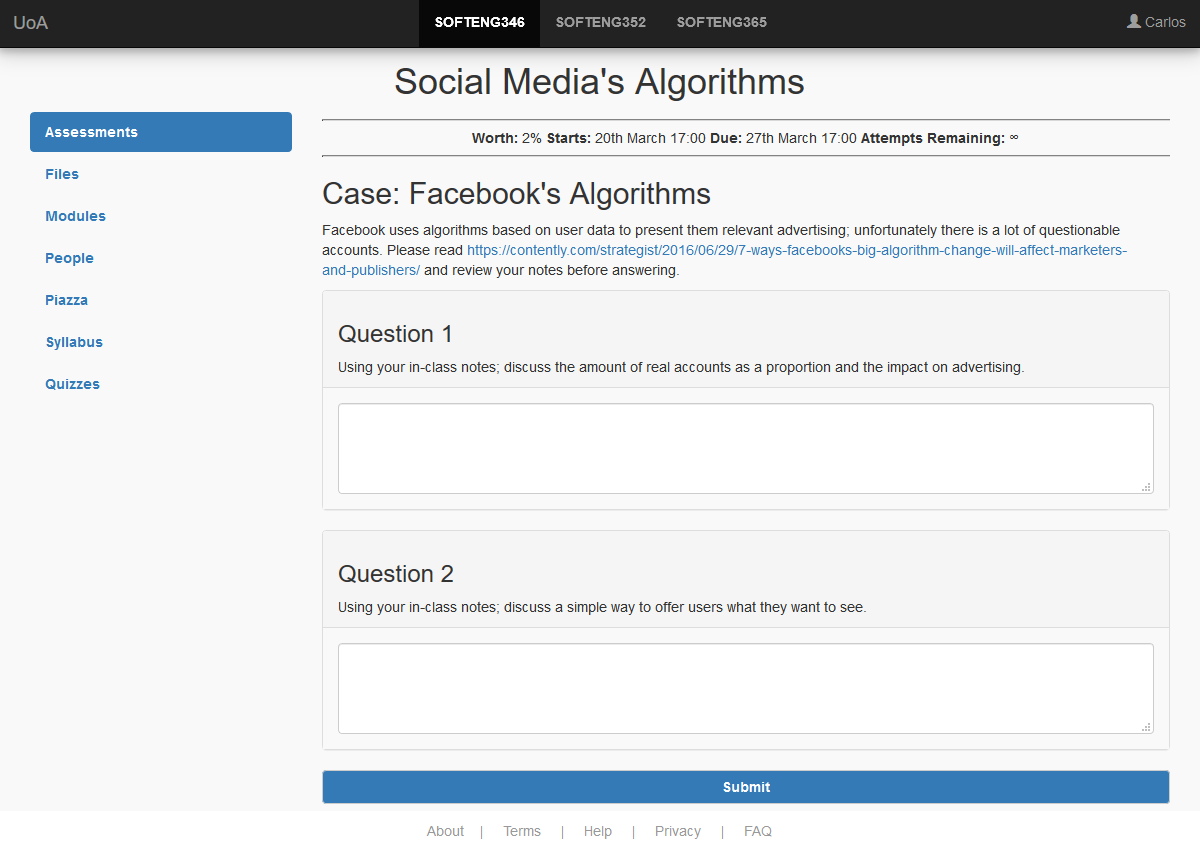
\includegraphics[width=\textwidth]{1 - Social Medias Algorithms.PNG}
		\caption{filling in the case with structured questions}
		\label{fig:one}
	\end{figure}
	\begin{figure}[H]
		\centering
		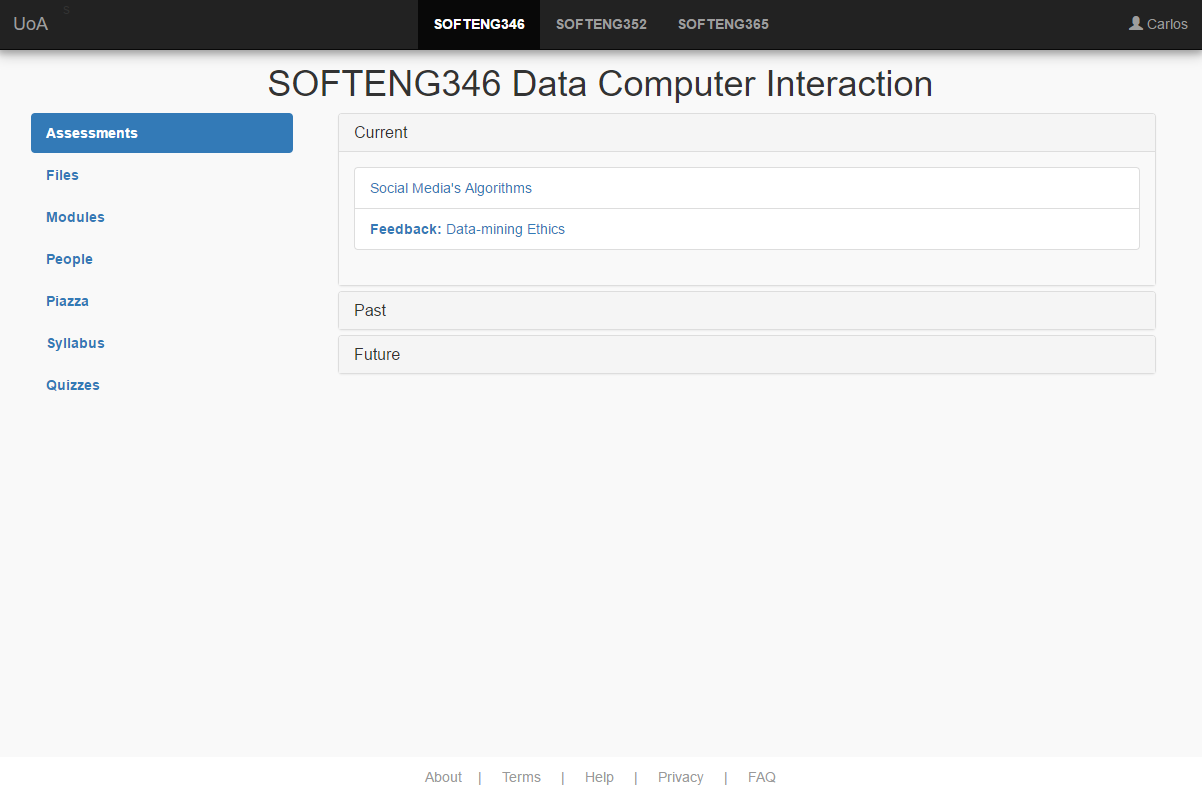
\includegraphics[width=\textwidth]{2 - Assessments (Current).PNG}
		\caption{list of assignments; specifically the current ones}
		\label{fig:two}
	\end{figure}
	\begin{figure}[H]
		\centering
		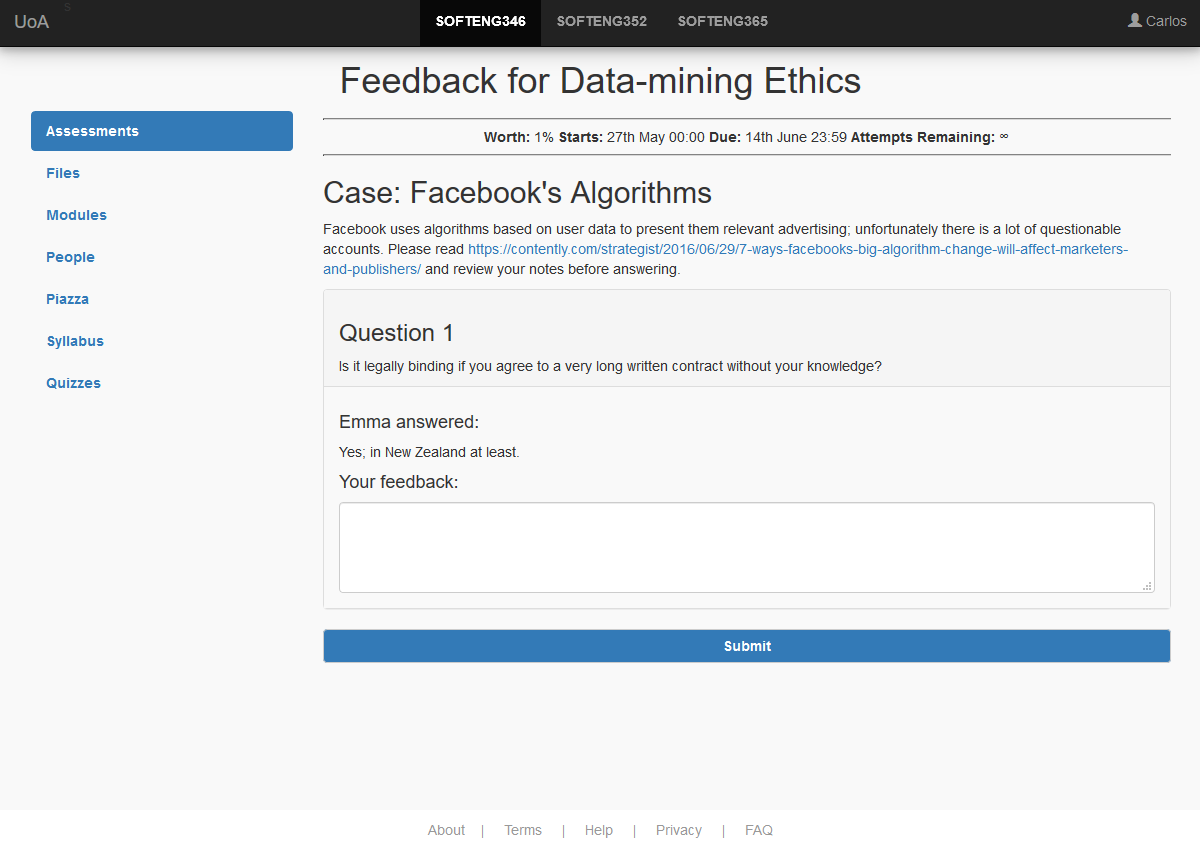
\includegraphics[width=\textwidth]{3 - Feedback for Data-mining Ethics.PNG}
		\caption{filling in feedback for another class peer}
		\label{fig:three}
	\end{figure}
	\begin{figure}[H]
		\centering
		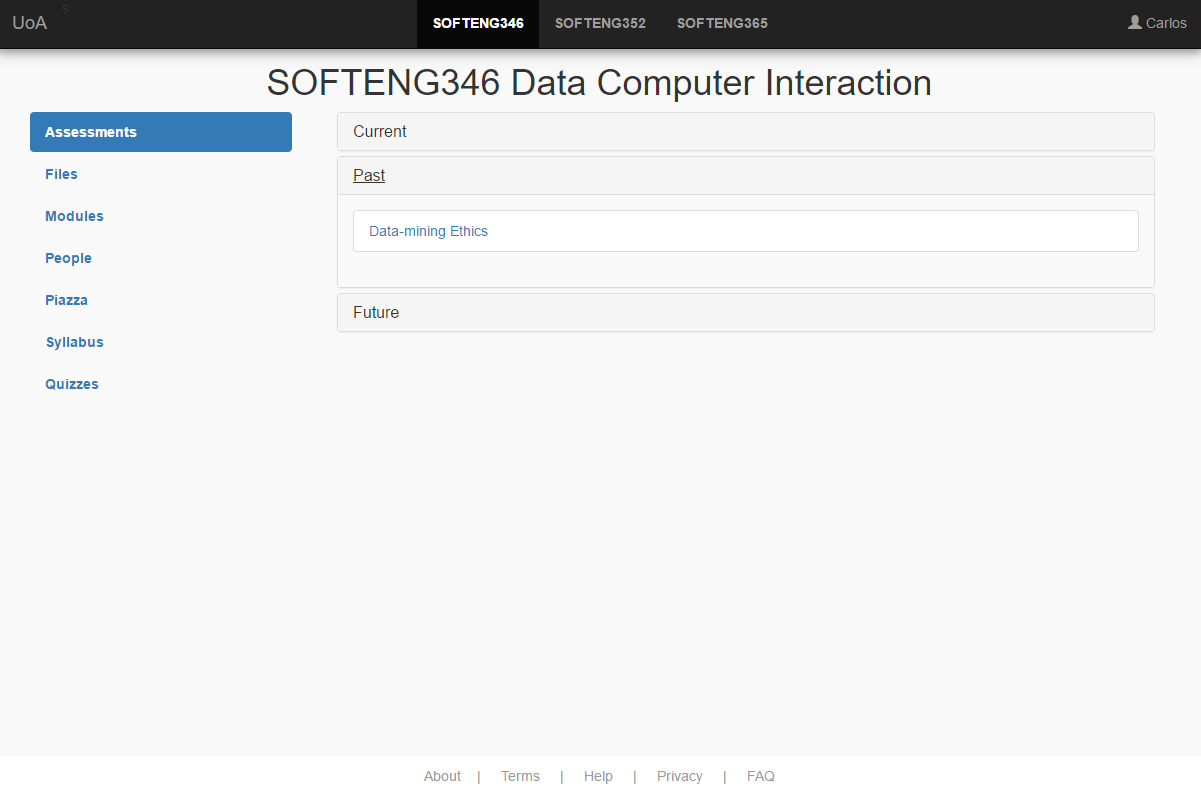
\includegraphics[width=\textwidth]{4 - Assessments (Past).PNG}
		\caption{list of assignments; specifically the previously submitted ones}
		\label{fig:four}
	\end{figure}
	\begin{figure}[H]
		\centering
		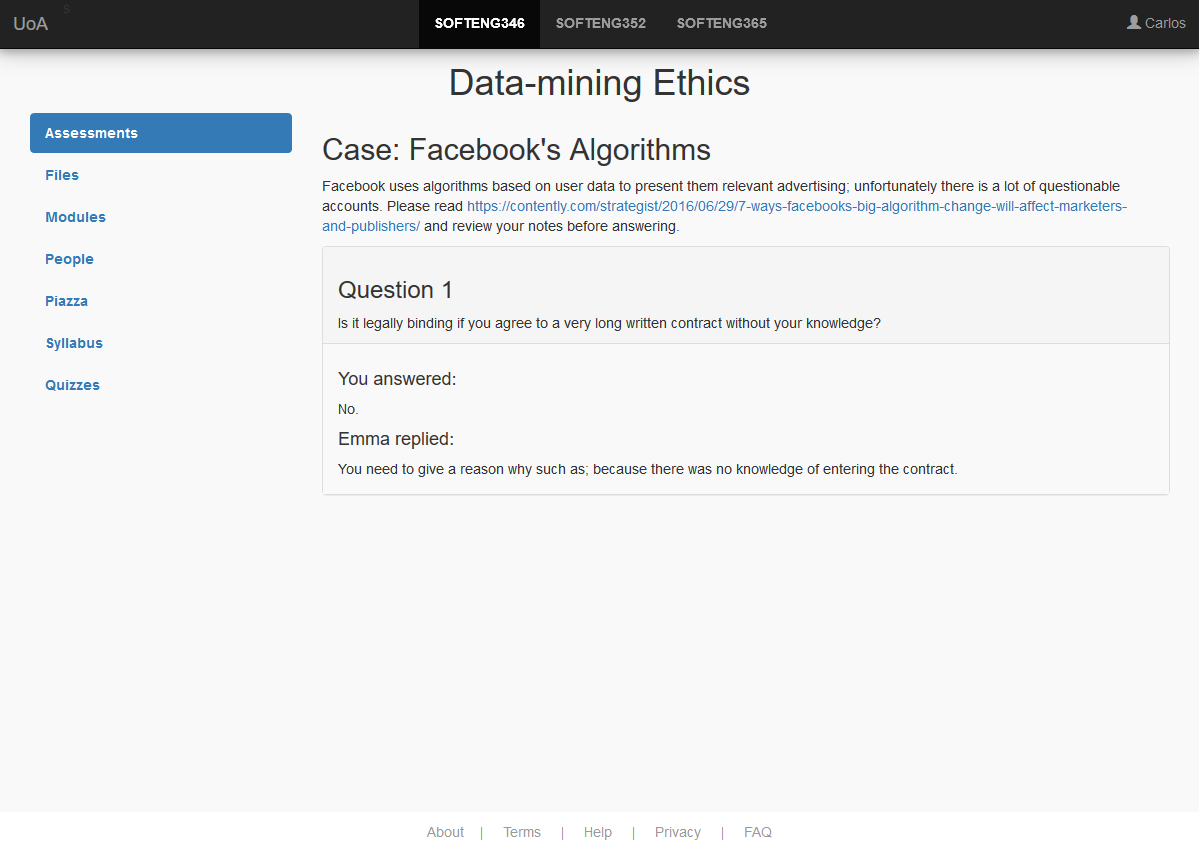
\includegraphics[width=\textwidth]{5 - Data-mining Ethics.PNG}
		\caption{reviewing another peer's feedback to the user}
		\label{fig:five}
	\end{figure}

	\subsection*{Out of Scope}
	Due to time constraints, irrelevancy, the fact this is a prototype and technical limitations there are some things which are out of scope. This fall into two categories:
		\subsubsection*{UI not implemented}
			\begin{itemize}
				\item WYSIWYG editors were not implemented because of the complexity of saving formatted text without a back-end and it's inappropriate for the short nature of the example questions.
				\item Other question types like check-boxes and MCQs were not implemented due to saving without a backend and it doesn't further illustrate the point of the prototype (it is possible).
				\item Tool-tips were not included as there are no features thought to be too complex or without labels to understand.		
				\item A quickly dismissed or disappearing banner or alert to show answers or feedback being saved before redirection back to assessments (requires a back-end or a more complex prototype).
				\item Real time use of two users to see feedback appearing after being given due to needing a back end or becoming too complex for a prototype.
			\end{itemize}
		\subsubsection*{UI implemented}
			\begin{itemize}
				\item Viewing other courses (``SE365'' and ``SE352'')
				\item Viewing and modifying personal settings/profile page
				\item `Home' button (``UoA'').
				\item All of the footer links and pages
				\item Text boxes for feedback and answers can't be limited to only resizing vertically due to a bug in bootstrap and the layout of the document.
				\item Viewing other categories for a course (``Files'', ``Modules'', ``People'', ``Piazza'', ``Syllabus'', and ``Quizzes'')
			\end{itemize}
			
		
\section{Colour Scheme}
	The prototype uses a monochrome on grey-scale colour scheme as seen in \cref{fig:color}
	\begin{figure}[H]
		\centering
		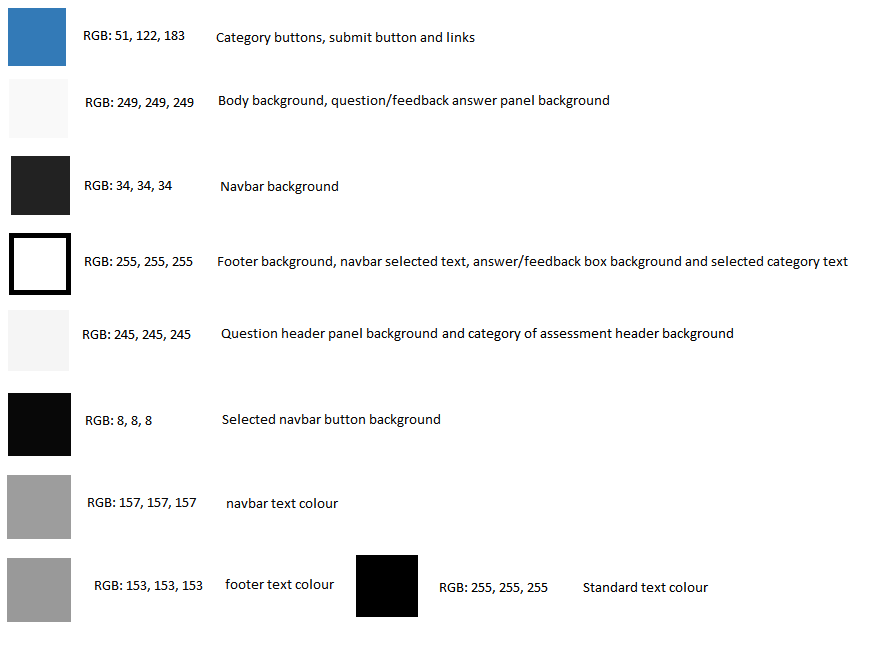
\includegraphics[width=\textwidth]{Colors.PNG}
		\caption{colour palette used for prototype}
		\label{fig:color}
	\end{figure}
	The palette was kept simple for a formal look with the minimal use of the blue for it to add character and emphasise what it is used on while ensuring easy reading. Blue that is a little darker was also used for the same reasons. Blue being on the lower end of the spectrum has another benefit of being less straining on the eye.\\
	
	High contrast was used to keep most of the text readable; however, the background is slightly grey to minimise strain on the eye. High contrast is also utilised between the navigation bar (navbar) and body of the website to distinguish them. Inverting the high contrast was used for buttons that have been selected to emphasise that fact.  The heading text is specifically black so that (in combination with being large at the top of the page) it is at the top of the contrast hierarchy; users look at it first so they know where they are.\\	
	
	Low contrast was used between the navbar components and footer components to help hide them so they are less distracting. Low contrast was also used to separate boxes so there is a visual distinguishable difference without distracting.
	
	
\section{Borders Scheme}
	100-250
	\begin{itemize}
		\item the horizontal rules around the submission details
		\item footer to main
		\item nav to header
		\item header to main
		\item sidebar to content
		\item | between the footer items
	%	\item box-shadow\: 0 4px 8px 0 rgba(0, 0, 0, 0.2), 0 6px 20px 0 rgba(0, 0, 0, 0.19); from \url{https://www.w3schools.com/css/css3_shadows.asp}
	\end{itemize}
	
	
\section{Fonts Scheme}
	\begin{figure}[H]
		\centering
		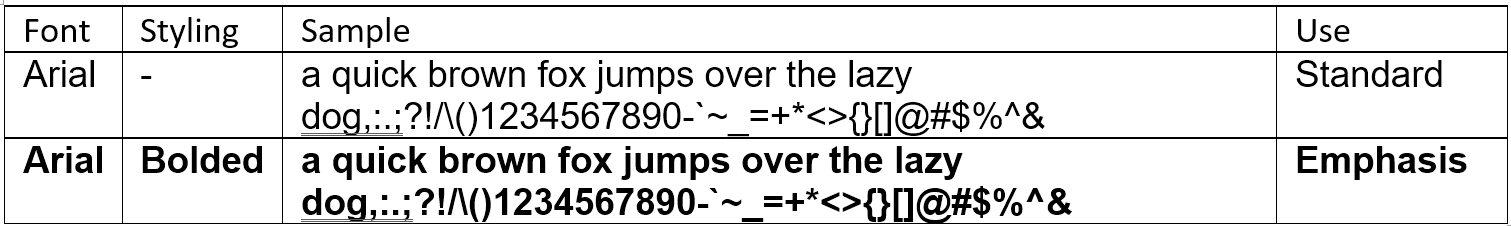
\includegraphics[width=\textwidth]{Fonts.PNG}
		\caption{font selection used for prototype}
		\label{fig:color}
	\end{figure}
		It is very important the user can read a lot in this system without strain as they could read a huge amount. Thus Arial was used throughout the prototype by letting all browsers use their default as it is the default for almost all the big browsers (it must be good enough for the experts at Google). Being a proportional font the speed and ease of reading is increased because users can distinguish the shape of whole words rather than having to read individual letters.\\
	
	Picking Arial means just using the browser's default so that allows the user to change the font when they change the default font in their browser if they prefer something else. Being a very popular font is available in almost every browser/OS combination and is default because it is so readable, easy on the eyes and modern. \\
	
	Bold text was used to distinguishing smaller headings instead of using font size to avoid to keep the size differences obvious. Bold text was also used in button text to distinguish it as a button, the extra emphasis informs the user that it's not just any old text.
	
	
\section{Resources Used}
	\subsection*{bootstrap}
		\begin{itemize}
			\item nawbar
			\item person glyphicon
			\item search for glyphicons
			\item look at classes (go through with a class equals "
		\end{itemize}
\end{document}
%https://piazza.com/class/iw7ylbqrrti7i?cid=243
%https://piazza.com/class/iw7ylbqrrti7i?cid=240

%user interacts with answer boxes to make them bigger